\paragraph{RV32M Multiply Extensi}

RV32M cung cấp các lệnh toán học để hỗ trợ các phép toán số nguyên phức tạp. Phần mở rộng này được thiết kế nhằm cải thiện hiệu suất cho các ứng dụng cần thực hiện nhiều phép tính số học như xử lý tín hiệu số và mật mã học.
\\
\textit{Các loại lệnh trong RV32M:}

\begin{itemize}
    \item \textit{Phép nhân (MUL):} Thực hiện phép nhân số nguyên giữa hai toán hạng, kết quả được lưu trong thanh ghi đích.
    \item \textit{Phép nhân giữ phần cao (MULH, MULHSU, MULHU):} Cung cấp kết quả phần cao từ các phép nhân:
    \begin{itemize}
        \item \textit{MULH:} Nhân hai số nguyên có dấu.
        \item \textit{MULHSU:} Nhân số nguyên có dấu với số nguyên không dấu.
        \item \textit{MULHU:} Nhân hai số nguyên không dấu.
    \end{itemize}
    \item \textit{Phép chia (DIV, DIVU):} Thực hiện phép chia số nguyên:
    \begin{itemize}
        \item \textit{DIV:} Chia hai số nguyên có dấu.
        \item \textit{DIVU:} Chia hai số nguyên không dấu.
    \end{itemize}
    \item \textit{Phép lấy dư (REM, REMU):} Lấy phần dư từ phép chia:
    \begin{itemize}
        \item \textit{REM:} Phần dư từ phép chia hai số nguyên có dấu.
        \item \textit{REMU:} Phần dư từ phép chia hai số nguyên không dấu.
    \end{itemize}
\end{itemize}



\paragraph{RV32A Atomic Extension}

RV32A  cung cấp các lệnh nguyên tử để hỗ trợ đồng bộ hóa giữa các tiến trình trong môi trường đa luồng. Các lệnh này đảm bảo rằng các thao tác đọc, sửa đổi và ghi vào bộ nhớ được thực hiện một cách an toàn, không bị gián đoạn, giúp duy trì tính nhất quán của dữ liệu. RV32A cung cấp hai loại lệnh nguyên tử chính:

\begin{itemize}
    \item \textit{Atomic Memory Operation (AMO):} Các lệnh này thực hiện thao tác nguyên tử trên dữ liệu trong bộ nhớ, bảo vệ dữ liệu khỏi những thay đổi không mong muốn trong suốt quá trình thực hiện.
    \item \textit{Load Reserved (LR) và Store Conditional (SC):} 
    \begin{itemize}
        \item \textit{LR}: Lệnh này đọc một \textit{word} từ bộ nhớ và đánh dấu địa chỉ bộ nhớ để theo dõi.
        \item \textit{SC}: Lệnh này lưu trữ một \textit{word} tại địa chỉ thanh ghi, nhưng chỉ thực hiện nếu địa chỉ bộ nhớ đã được đánh dấu bởi lệnh \textit{LR}, giúp đồng bộ hóa hiệu quả giữa các tiến trình.
    \end{itemize}
\end{itemize}

\begin{figure}[!h]
    \centering
    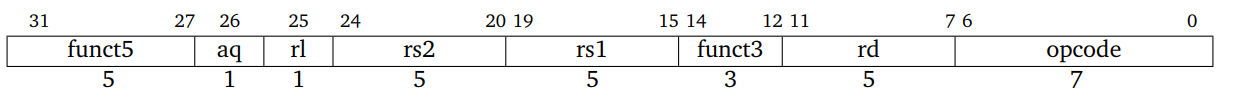
\includegraphics[width=6in]{Images/Risc-V/RV32A.png}
    \vspace{10pt} % Thay đổi giá trị 10pt theo nhu cầu
    \caption{RV32A Instruction Format}
\end{figure}

% Trong RV32A, các lệnh Atomic Memory Operations (AMO) và Load Reserved (LR) / Store Conditional \
% (SC) bao gồm:

% \begin{itemize}
%     \item \textbf{lr.w} - Load Reserved: Đọc từ bộ nhớ và đánh dấu địa chỉ.
%     \item \textbf{sc.w} - Store Conditional: Lưu dữ liệu vào bộ nhớ nếu đã được đánh dấu.
%     \item Các lệnh AMO: \textbf{amoswap.w}, \textbf{amoadd.w}, \textbf{amoand.w}, \textbf{amoor.w}, \textbf{amoxor.w}, \textbf{amomax.w}, \textbf{amomaxu.w}, \textbf{amomin.w}, \textbf{amominu.w}.
% \end{itemize}

% Những lệnh này giúp thực hiện các thao tác nguyên tử trên bộ nhớ, đảm bảo đồng bộ hóa và tính nhất quán trong môi trường đa luồng. Các lệnh nguyên tử trong RV32A đóng vai trò quan trọng trong việc phát triển các ứng dụng đa luồng và hệ thống nhúng, giúp tăng cường hiệu suất và bảo vệ dữ liệu một cách an toàn, hiệu quả.


\paragraph{RV32F / D Floating-Point Extensions }

RV32F / D cung cấp các lệnh hỗ trợ tính toán số thực tuân theo tiêu chuẩn IEEE 754, nhằm đáp ứng nhu cầu tính toán chính xác trong các ứng dụng khoa học và kỹ thuật. Các lệnh này cho phép xử lý hiệu quả dữ liệu số thực dấu phẩy động, bao gồm cả định dạng \textit{single-precision} (32-bit) và \textit{double-precision} (64-bit). RV32F / D cung cấp hai nhóm lệnh chính:

\begin{itemize}
    \item \textit{Phép toán số thực cơ bản:}  
    Các lệnh này thực hiện các phép tính cơ bản trên số thực, bao gồm cộng, trừ, nhân, chia, căn bậc hai và các phép so sánh, giúp xử lý hiệu quả các tác vụ tính toán phức tạp.

    \item \textit{Chuyển đổi định dạng:}  
    \begin{itemize}
        \item \textit{Từ số nguyên sang số thực:} Hỗ trợ chuyển đổi dữ liệu giữa số nguyên và số thực (32-bit hoặc 64-bit).  
        \item \textit{Giữa single và double precision:} Hỗ trợ chuyển đổi định dạng giữa hai loại số thực, phù hợp với yêu cầu ứng dụng.
    \end{itemize}
\end{itemize}
\\

\textit{Cơ chế đặc biệt:}  
\begin{itemize}
    \item \textit{Thanh ghi số thực:} Cung cấp 32 thanh ghi số thực (\texttt{f0} đến \texttt{f31}), kích thước 32-bit (RV32F) hoặc 64-bit (RV32D).
    \item \textit{Kiểm soát trạng thái ngoại lệ:} Các cờ trạng thái để phát hiện và xử lý các tình huống như tràn, chia cho 0 hoặc số không hợp lệ.
\end{itemize}
\\
\begin{figure}[!h]
    \centering
    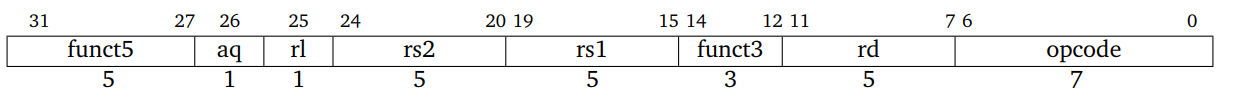
\includegraphics[width=6in]{Images/Risc-V/RV32A.png}
    \vspace{10pt} % Thay đổi giá trị 10pt theo nhu cầu
    \caption{RV32F / D Instruction Format}
\end{figure}
RV32F / D được sử dụng rộng rãi trong các ứng dụng yêu cầu tính toán số thực chính xác, như trí tuệ nhân tạo, xử lý hình ảnh, và mô phỏng khoa học, giúp nâng cao hiệu suất và tính linh hoạt của hệ thống.



\paragraph{RV32C Compressed Extension}
RV32C cung cấp các lệnh nén nhằm giảm kích thước mã lệnh và cải thiện hiệu quả sử dụng bộ nhớ trong các hệ thống nhúng hoặc ứng dụng yêu cầu bộ nhớ hạn chế. Phần mở rộng này hỗ trợ một tập hợp con các lệnh RISC-V, được mã hóa bằng 16-bit thay vì 32-bit, giúp giảm kích thước mã lệnh một cách đáng kể mà vẫn đảm bảo hiệu suất. 
\\
\\
\textit{Các tính năng chính:}
\begin{itemize}
    \item \textit{Giảm kích thước mã lệnh:}  
    RV32C sử dụng các lệnh nén 16-bit, giúp tiết kiệm bộ nhớ chương trình, đặc biệt hữu ích trong các ứng dụng nhúng và IoT.

    \item \textit{Khả năng tương thích:}  
    Các lệnh nén được thiết kế để tương thích với các lệnh 32-bit, cho phép thực thi trên cùng một kiến trúc mà không cần thay đổi phần cứng.

    \item \textit{Tối ưu hóa hiệu suất:}  
    Việc giảm kích thước mã lệnh giúp cải thiện khả năng sử dụng bộ nhớ đệm và giảm băng thông bộ nhớ, từ đó tăng hiệu suất tổng thể của hệ thống.
\end{itemize}
\textit{Phân loại các lệnh nén:}
\begin{itemize}
    \item \textit{Nén tải và lưu trữ:}  
    Cung cấp các lệnh nén để thực hiện các thao tác tải (\texttt{C.LW}, \texttt{C.LD}) và lưu trữ (\texttt{C.SW}, \texttt{C.SD}) dữ liệu.

    \item \textit{Nén các phép toán số học:}  
    Các lệnh như \texttt{C.ADD}, \texttt{C.SUB} hỗ trợ thực hiện các phép toán số học cơ bản.

    \item \textit{Nén điều kiện nhánh:}  
    Cung cấp các lệnh nén để xử lý nhánh như \texttt{C.BEQZ}, \texttt{C.BNEZ}, giúp giảm kích thước mã điều kiện
\end{itemize}
\begin{figure}[!h]
    \centering
    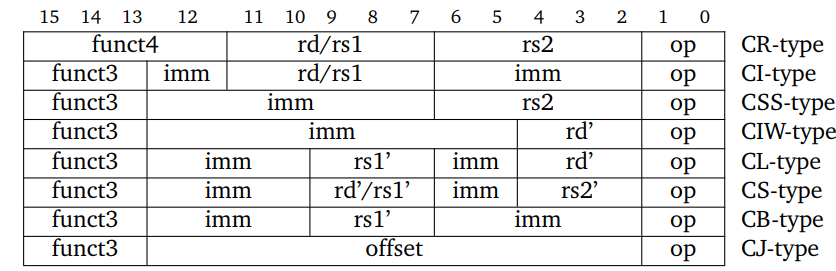
\includegraphics[width=6in]{Images/Risc-V/RV32C.png}
    \vspace{10pt} % Thay đổi giá trị 10pt theo nhu cầu
    \caption{RV32C Instruction Format}
\end{figure}
RV32C là một lựa chọn tối ưu cho các hệ thống yêu cầu mật độ mã cao, chẳng hạn như các thiết bị IoT, hệ thống nhúng và các ứng dụng yêu cầu tiết kiệm năng lượng.
